Per distillazione si intende la tecnica utilizzata per separare due o più sostanze presenti in una miscela. Essa sfrutta la differenza dei punti di ebollizione di tali sostanze, cioè la loro differenza di volatilità.

\vspace{-0.3cm}\subsection{Distillazione a P costante di soluzioni ideali}
Nei tre grafici precedenti avevamo la frazione molare in ascisse e la pressione in ordinate. Consideriamo adesso un grafico avente la frazione molare in ascisse e T in ordinate:

\vspace{-0.5cm}\begin{figure}[H]
    \centering
    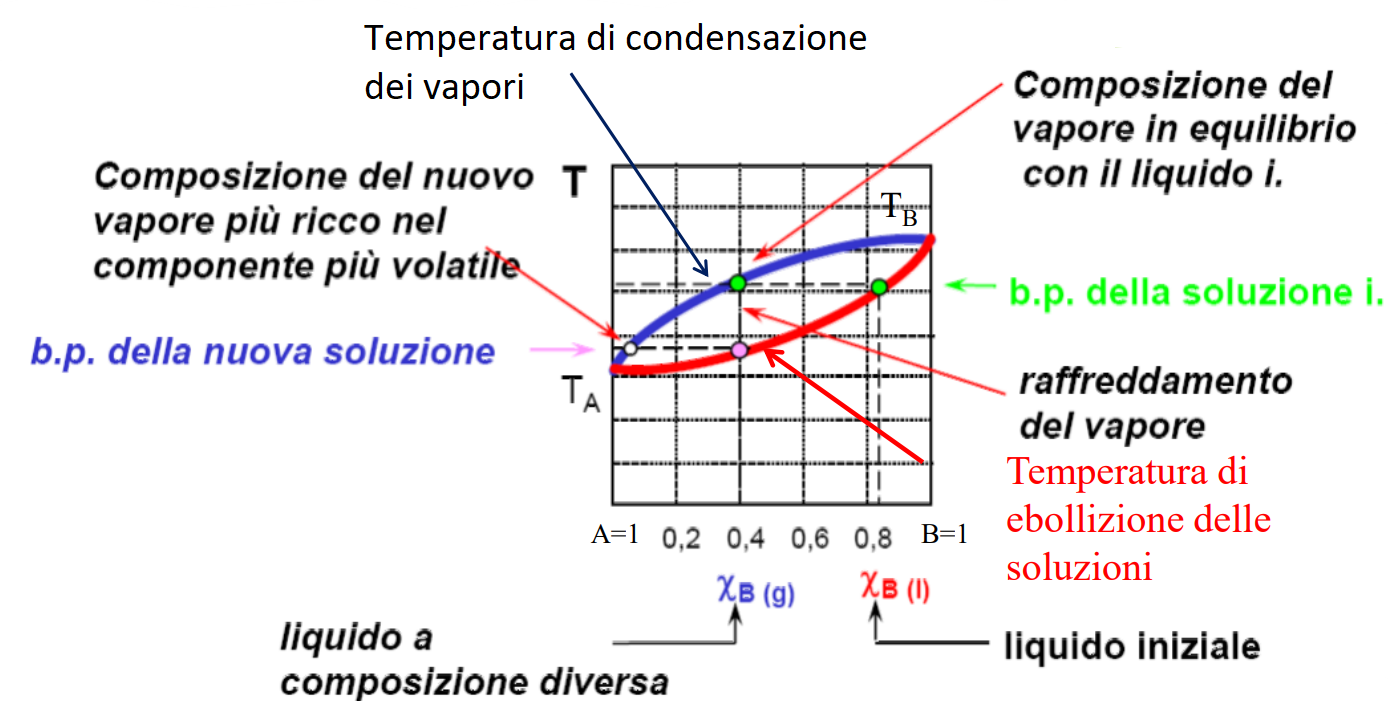
\includegraphics[width=14.3cm]{immagini/distillazione_ideale.png}
\end{figure}

Spesso in natura abbiamo delle soluzioni e il nostro obiettivo è separarle (ad es. il petrolio), ossia si vuole sfruttare la diversa volatilità di sostanze che si trovano in soluzione per separarle.

Il caso più semplice è quello di una soluzione formata da una specie A e una specie B. Graficamente avremo che in basso a sinistra la frazione molare di A è 1 e quella di B è 0, viceversa in basso a destra la frazione molare di B è 1 e quella di A è 0. Nei punti intermedi avremo invece tutte le infinite composizioni della miscela possibili.

Va da notare che i grafici sono sperimentali.

$T_A$ è la temperatura di ebollizione del componente A puro, $T_B$ quella del componente B puro.

Dal grafico si evince che B è meno volatile di A, infatti ha una temperatura di ebollizione più alta.

La linea rossa indica le diverse temperature di ebollizione delle varie soluzioni, quindi ogni soluzione AB avente la sua specifica composizione avrà una sua particolare temperatura di ebollizione; la linea blu invece indica la temperatura di condensazione dei vapori aventi le diverse composizioni. Il motivo per cui rappresentiamo queste due linee è che se vogliamo distillare l'obiettivo è quello di raccogliere poi il distillato e farlo condensare.

Supponiamo di avere una certa composizione della soluzione (nel disegno indicata dal punto verde sulla linea rossa) e iniziamo a riscaldare. La temperatura aumenterà fino a raggiungere la temperatura di ebollizione della soluzione, per cui la soluzione bolle, cioè la tensione di vapore ha eguagliato la pressione atmosferica (o in generale la pressione esterna). Inoltre da questo momento in poi fin quando  tutto il liquido non diventa vapore la temperatura non aumenta più. Allora si parla di \textit{calore latente di evaporazione}.

Dato che la soluzione sta bollendo abbiamo ottenuto dei vapori. Cosa abbiamo in fase vapore?

Ci si sposta orizzontalmente verso sinistra fino a trovare la curva blu. In questo modo la temperatura di condensazione del vapore è uguale alla temperatura di ebollizione, ma la composizione cambia: se raffreddiamo il vapore troveremo una composizione diversa da quella di partenza (indicata dal punto rosa sulla curva rossa).

Se riscaldiamo la nuova soluzione ottenuta per condensazione avremo una nuova temperatura di ebollizione. Se condensiamo il nuovo vapore dal grafico si evince che otterremo una soluzione composta quasi del tutto da A. Infatti per successive distillazioni si è in grado di ottenere A puro come distillato e B come residuo. Quindi se la soluzione ha comportamento ideale saremo in grado di separare, per successive distillazioni, i due componenti. In particolare il più volatile sarà nella fase vapore, il quale viene poi condensato; il meno volatile sarà nella fase liquida.

\E dunque possibile separare le soluzioni ideali nei loro componenti attraverso la distillazione. Il processo dovrà solo essere ripetuto perché di volta in volta i vapori saranno più ricchi nel componente più volatile.
\subsection{Distillazione di soluzioni reali}
Andiamo adesso a vedere cosa succede per soluzioni non ideali, cioè che deviano dalla legge di Raoult. Esse sono tutte quelle soluzioni per le quali le interazioni tra A e B sono o più deboli o più forti rispetto alle interazioni A-A e B-B, ossia quando $\Delta$H$>$0 o $\Delta$H$<$0. Anche in questo caso si ottengono grafici sperimentali.

\vspace{0.2cm}Consideriamo il caso in cui $\Delta$H$_{sol}$$<$0, cioè quello in cui la reazione è esotermica e quindi la soluzione emette calore.

Dal grafico si evince che la temperatura necessaria per far bollire e distillare ogni possibile soluzione si è alzata, quindi si deve fornire più energia. Il motivo è che le interazioni che si hanno nelle molecole in soluzione risultano essere più forti di quelle presenti tra le molecole nelle speci pure.

\begin{minipage}{0.4\textwidth}
    \begin{figure}[H]
        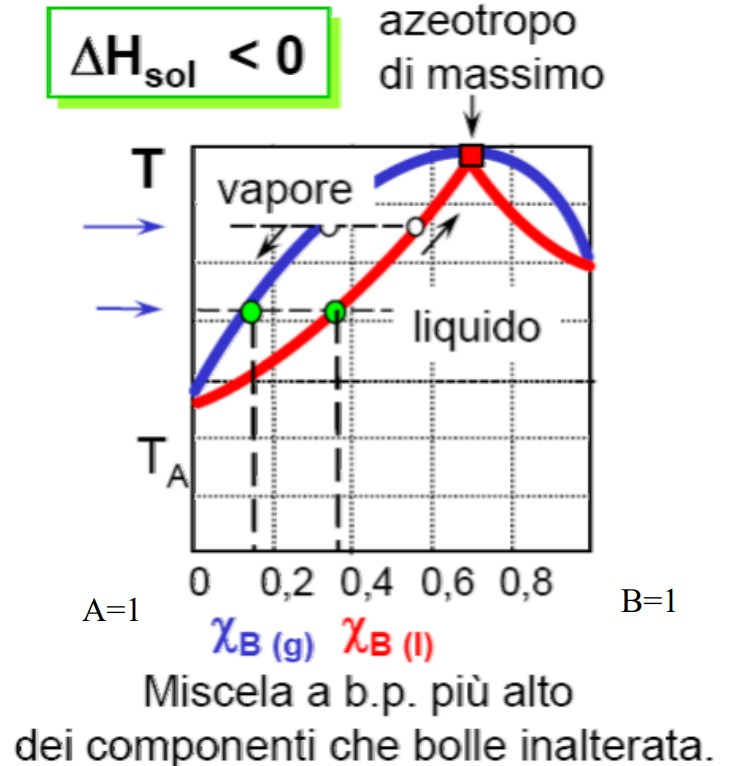
\includegraphics[width=6cm]{immagini/distillazione_esotermica.png}
    \end{figure}
\end{minipage}
\begin{minipage}{0.6\textwidth}
    \vspace{0.6cm}Presa una certa composizione, la riscaldiamo fino ad arrivare al punto sulla linea rossa che indica la temperatura di ebollizione. La soluzione inizierà a bollire e la composizione del vapore sarà ottenuta spostandoci orizzontalmente a sinistra. Si evince che nel vapore la quantità di A, rispetto a quella della soluzione liquida, è aumentata.

    Se A aumenta nella fase vapore significa che lo stiamo sottraendo alla fase liquida, quindi in quest'ultima avremo più B. Pertanto il vapore sta producendo A, mentre la soluzione si sta spostando a destra come composizione.
\end{minipage}

\vspace{0.3cm}Ci sarà un punto in cui la soluzione, cioè la fase liquida, raggiungerà la composizione corrispondente al quadrato rosso nel grafico. Tale punto è comune alla linea del liquido e a quella del vapore, ossia la composizione del liquido (che si sta arricchendo in B perché stiamo facendo evaporare A) diventa uguale alle composizione del vapore che distilleremo. A questo punto sarà inutile fare ulteriori distillazioni, perché si è arrivati alla \textbf{composizione azeotropica}, cioè si è formato un \textbf{azeotropo}, ossia una soluzione che bolle inalterata (cioè la composizione di liquido e vapore sono uguali).

Otterremo quindi l'azeotropo come residuo e A puro come distillato.

Abbiamo fatto un esempio in cui partivamo da una composizione a sinistra dell'azeotropo, adesso partiamo da una composizione a destra di questo.

In questo caso, dopo aver portato all'ebollizione la soluzione, la composizione del vapore si otterrà spostandoci orizzontalmente verso destra, cioè il vapore sarà più ricco in B. Se però sottraiamo B dalla soluzione, quest'ultima si arricchirà in A. In altre parole avremo B nella fase vapore e una soluzione avente composizione con meno B che quindi si sposta verso sinistra.

Con successive distillazioni avremo B puro come distillato e l'azeotropo come residuo.

Quindi, qualunque sia la composizione dalla quale partiamo, possiamo ottenere, a seconda se ci troviamo a sinistra o a destra dell'azeotropo, rispettivamente, A puro come distillato e l'azeotropo come residuo oppure B puro come distillato e ancora l'azeotropo come residuo, ossia si riesce a separare solo una parte di un componente e si può fino a quando non otteniamo in soluzione una composizione che è quella azeotropica, che ritroviamo nella fase vapore.

Questo è il problema per cui, ad esempio, per distillazione tra acqua e alcol non è mai possibile, pur essendo l'alcol più volatile, ottenere l'alcol "assoluto" cioè puro. Tuttavia l'alcol puro è comune in laboratorio. Come si fa?

Si distilla acqua ed alcol reiterando il processo fino a quando raggiungiamo l'azeotropo, per cui ci si deve fermare. Si prende allora questa soluzione (che non è più possibile separare nei suoi componenti) composta da tanto alcol e dalla poca acqua che non siamo riusciti a separare, e la si fa reagire con ossido di calcio. L'ossido assorbirà l'acqua residua diventando idrossido, quindi ora il problema sarà separare alcol e idrossido di calcio, che è un solido gelatinoso. Per fare ciò si adoperano altri metodi che eludono dai nostri studi.

\vspace{0.2cm}Consideriamo adesso una soluzione con $\Delta$H$>$0, cioè il processo di dissoluzione è endotermico e bisogna dunque fornire energia altrimenti la soluzione non si forma. Ciò significa che le interazioni tra A e B sono deboli rispetto a quelle che si esercitavano nei liquidi puri e infatti tutte le possibili soluzioni avranno temperature di ebollizione più basse.

\vspace{-0.2cm}\begin{minipage}{0.4\textwidth}
    \begin{figure}[H]
        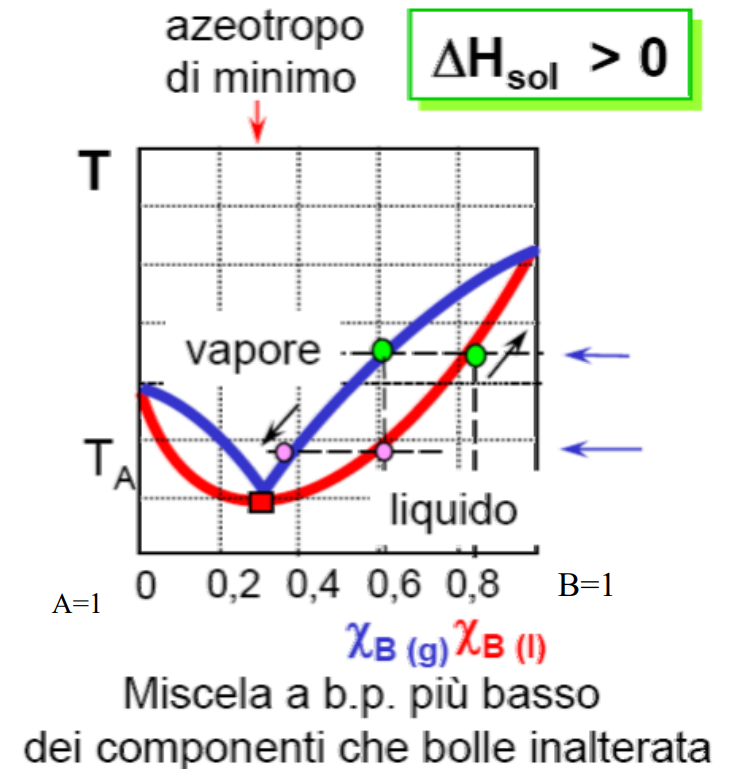
\includegraphics[width=6cm]{immagini/distillazione_endotermica.png}
    \end{figure}
\end{minipage}
\begin{minipage}{0.6\textwidth}
    \vspace{0.6cm}Immaginiamo di essere a destra dell'azeotropo e di avere una certa composizione. Riscaldiamo la soluzione fino a quando inizia a produrre vapore, il quale avrà una diversa composizione (più a sinistra). Condensandola troviamo una nuova soluzione, più vicina all'azeotropo.

    Quindi succede il contrario del caso precedente, cioè mentre prima il vapore ci dava A puro o B puro a seconda che ci trovassimo a destra o a sinistra dell'azeotropo, ora invece sarà il vapore ad avvicinarsi alla composizione azeotropica, pertanto stavolta avremo l'azeotropo come distillato e il componente puro come residuo.
\end{minipage}

\vspace{0.2cm}In sintesi, se ci troviamo alla destra dell'azeotropo avremo l'azeotropo come distillato e B puro come residuo, se ci troviamo alla sua sinistra otterremo l'azeotropo come distillato e A puro come residuo.

\vspace{0.2cm}Recap: discutendo la legge di Raoult, valida per soluzioni ideali, abbiamo visto che la tensione di vapore di queste è funzione della loro composizione. Si hanno quindi dei diagrammi con frazione molare sulle ascisse e tensione di vapore sulle ordinate. Questi sono grafici validi per temperature fissate.

Ci siamo chiesti se, presa una soluzione formata da due componenti, sia possibile separare i due liquidi. Ciò è possibile solo per soluzioni ideali.

Abbiamo allora considerato dei grafici a pressione costante, con la frazione molare sulle ascisse e la temperature sulle ordinate. Da essi si evince che qualunque sia la composizione iniziale è possibile ottenere, per successive distillazioni, i componenti puri.

Viceversa per le soluzioni non ideali non è possibile ottenere entrambi i componenti del tutto puri, ma di norma si ottiene uno dei due puro mentre l'altro si ottiene con una composizione detta azeotropica.

Abbiamo affrontato il caso in cui l'entalpia di mescolamento $\Delta$H sia positiva e il caso in cui sia negativa. Queste soluzioni sono dovute al fatto che le interazioni tra le molecole di A e quelle di B risultano essere diverse da quelle che si esercitano nelle speci pure (per diverse si intende che sono più forti o più deboli). Per entrambi i casi abbiamo poi visto cosa succede se ci troviamo a sinistra o a destra dell'azeotropo. Si trova che distillando il vapore sarà più ricco in una componente e il residuo sarà di conseguenza più ricco nell'altra. Quest'ultimo tende ad andare verso la composizione azeotropica, in cui la miscela "non distilla più", nel senso che il vapore avrà la stessa composizione del liquido, quindi sarà inutile fare l'operazione di distillazione.